\chapter{Market Understanding and Data Selection}

This chapter, I will briefly illustrate the characteristics of Hong Kong stock market. After that, some introduction about the parameters I choose for this dissertation

\section{Introduction of Hong Kong Stock Exchange market}

\begin{figure}[h]
	\centering
	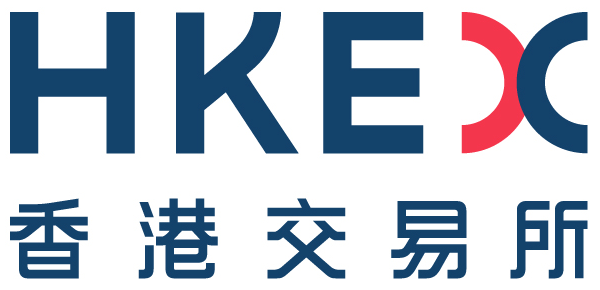
\includegraphics[width=0.4\textwidth]{hkexlogo}
	\caption{logo of HKEX}
\end{figure}

Hong Kong is one of the world’s leading financial centers with low taxation, near-free port trade, and international financial markets. Hong Kong is also the freest country all over the world\cite{freedom_ranking_2016}. Thus, even after the setbacks of Asian Financial Crisis and 1008 Global Economic Downturn, Hong Kong still have attracted a lot of international investors.\\

Hong Kong Exchanges and clearing Limited, or HKEX, is a stock exchange operator and clearing houses located in Hong Kong. Its ability of securities can be traced back to the foundation of the Association of Stockbrokers in Hong Kong in 1891\cite{1_history_hkex_markets_2016}.\\

HKEX is now one of the largest operators all over the world. By the end of 2015, there are 1866 companies listed on HSI, 951 of which are from mainland China, and HKEX’s total market capitalization is around HK\$24.68trillion and around 60\% of which are taken up by mainland companies. Number of trades is around 1.4million billion\cite{hkex_fact_book_2015}.\\

From the above figures, we can find that HKEX is an active exchange market and it also can be inferred that Mainland China have great influence on HKEX.\\

As a developed market, the efficiency of HKEX has already been proved \cite{su2015efficiency}. This give our study a great convenient.

\begin{figure}[h]
	\centering
	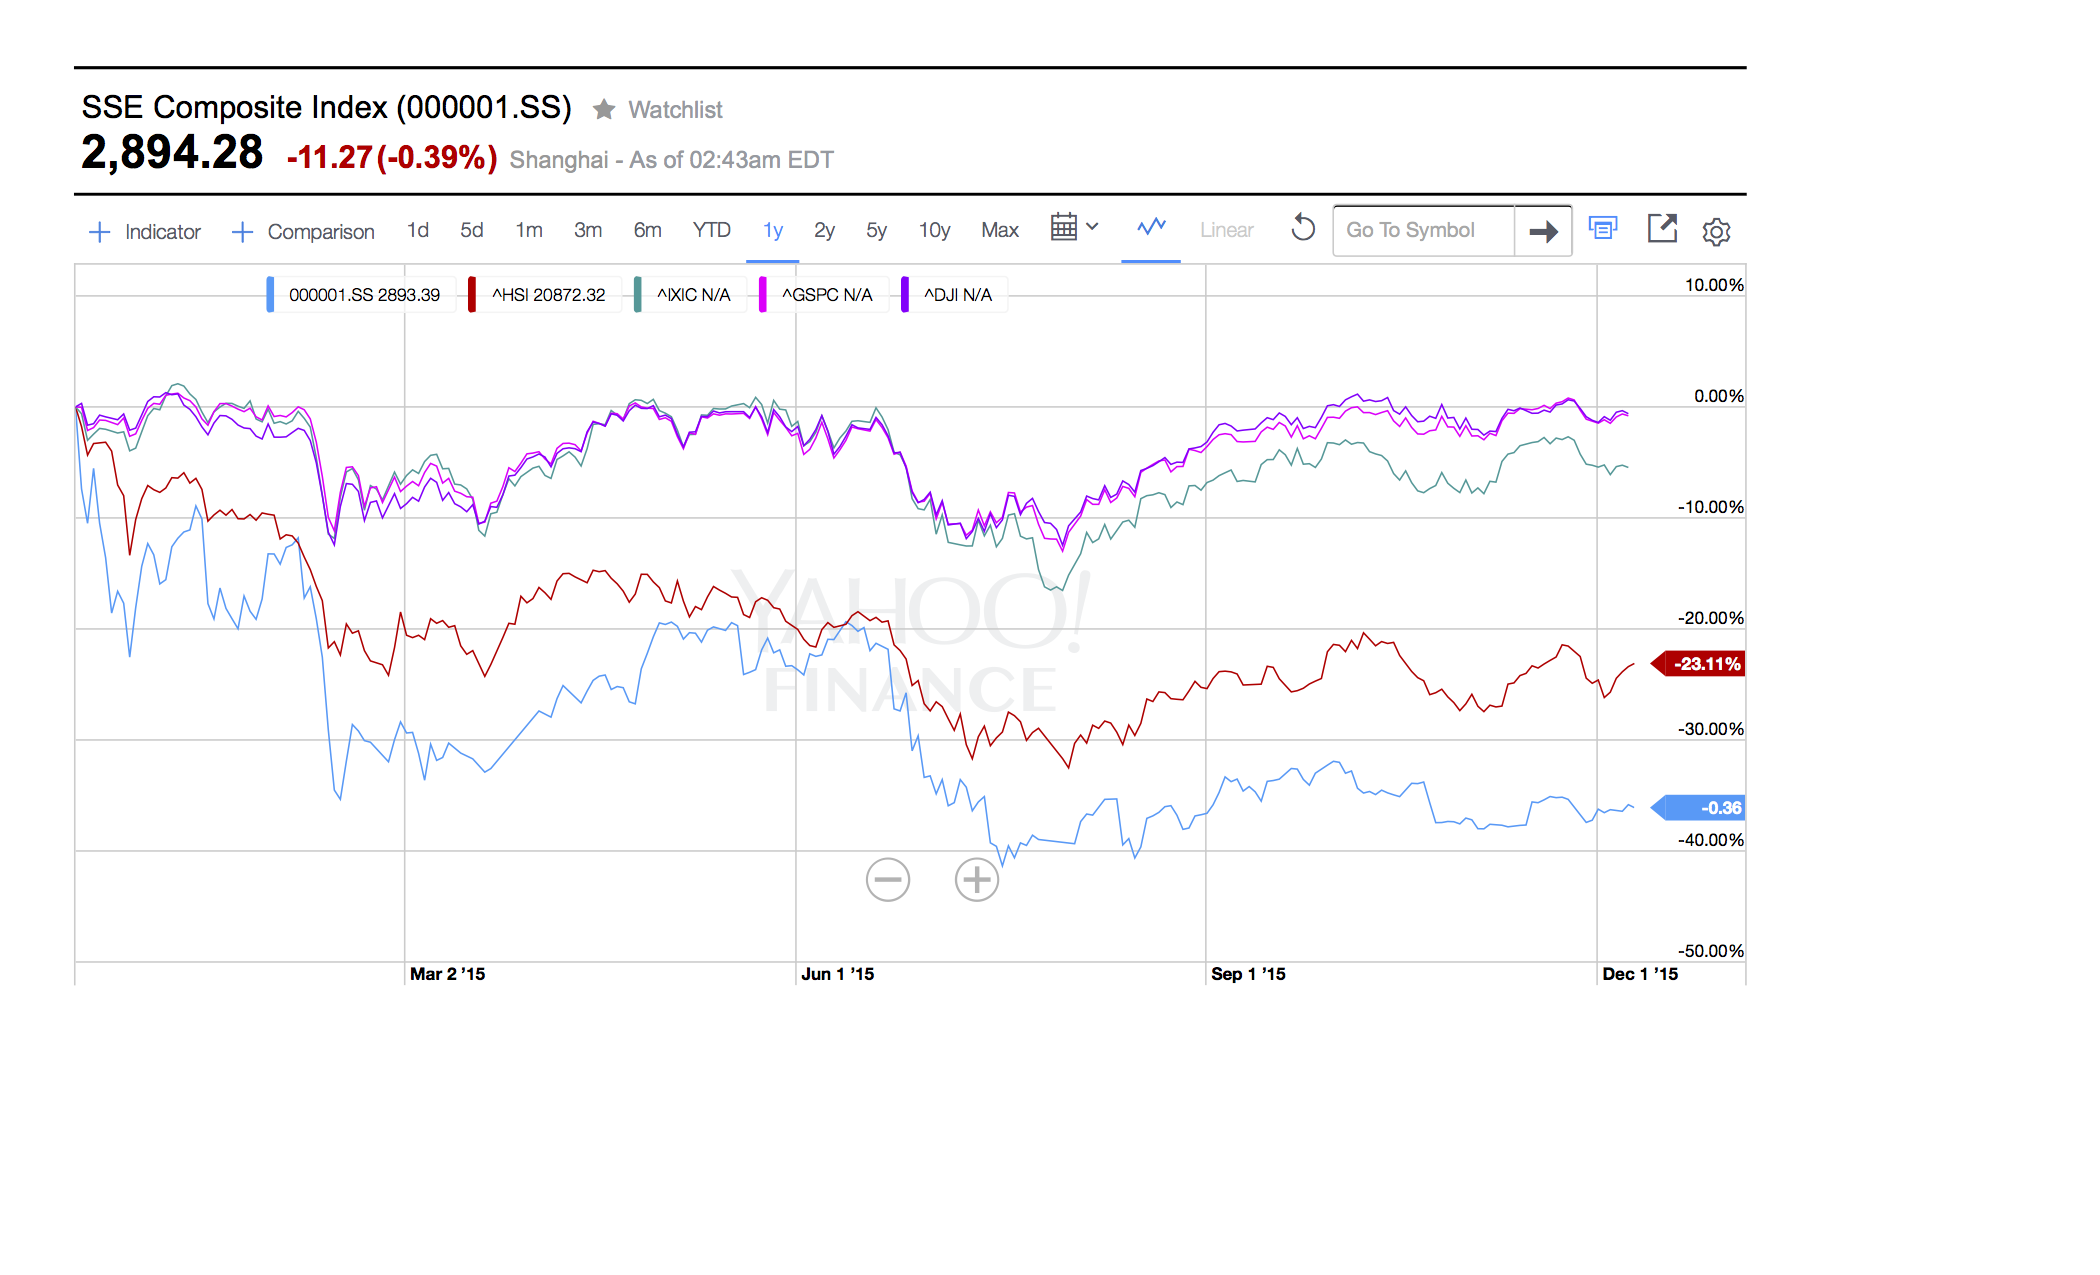
\includegraphics[width=0.8\textwidth]{lastyearhsi}
	\caption{Comparison of HSI and other indexes}
\end{figure}

Starting in 1969, Heng Seng Index, or HSI, is the most widely quoted gauge of the Hong Kong stock market\cite{hsi_company_profile}. This index includes the largest and most liquid stocks listed in Hong Kong, and there are four sub-indexes Finance, Utilities, Properties and Commerce \& Industry\cite{heng_seng_index}. Its base index is 100 point and nowadays is over 20,000 points.

\section{Data Selection}

My object is to predict the stock price, the following data are selected and would be used as input data to do further process. 

\subsection{Historical Price}
Based on the efficiency theory, past information affects stock price movements. In this experiment, I choose last transaction date price to be input, and use some other indicators to represent the stock change direction and other historical information.

\subsection{Technical Indicator}

Based on \cite{lauretto2013evaluation} the following indicators are used, calculated through ta-lib package (http://ta-lib.org/):
\begin{itemize}
	\item Simple moving average (SMA) of 3, 13 and 21 days
	\item Exponential moving average (EMA) of 5, 13 and 21 days
	\item Rate of Change (ROC) of 13 and 21 days
	\item Moving average convergence divergence (MACD) with short term moving average of 12 days and long term moving average of 26 days and with short term moving average of 7 days and long term moving average of 14 days
	\item Relative strength index (RSI) of 9, 14 and 21 days.
\end{itemize}

\subsection{Hang Seng Interbank Offered Rate (HIBOR)}
HIBOR is the annualized rate charged for interbank lending on HKD denominated instruments\cite{chen2010principal}. If HIBOR goes higher, then investors tend to leave stock market. As a result, stock price will decrease. HIBOR rate varies from overnight to one year. \\



In this experiment, one-week, one-month, half-year and one-year HIBOR are used. 

\begin{figure}[h]
	\centering
	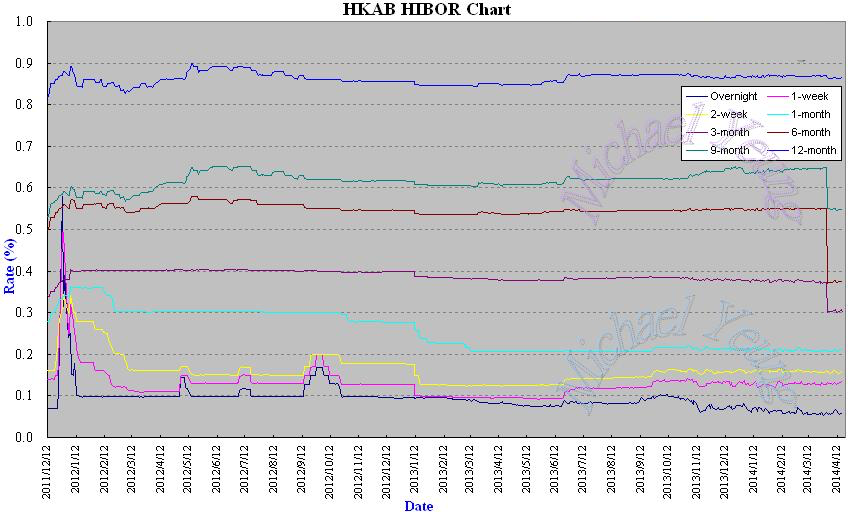
\includegraphics[width=0.8\textwidth]{HIBORChart}
	\caption{HIBOR from 2011 to 2014}
\end{figure}



\subsection{Foreign exchange rate}
Foreign exchange rate is the value of one country’s currency in terms of another currency. In \cite{ma1990exchange} Christopher and Kao found that changes of foreign exchange rate have impacts on stock price. As HKEX is a stock exchange has many international investors, stock prices changes greatly while the foreign exchange rate is volatile.\\


In this experiment, rates from CNY, USE, EUR to HKD are used.

\subsection{other data}
Daily level HSI and SSE data are also used. Besides, some ETF (includes iShares China Large-Cap, which composed of large-capitalization Chinese equities that trade on the Hong Kong Stock Exchange) prices are also taken into consideration.
